\documentclass[acmtog]{acmart}
\usepackage{graphicx}
\usepackage{subfigure}
\usepackage{natbib}
\usepackage{listings}
\usepackage{bm}
\usepackage{amsmath}

\definecolor{blve}{rgb}{0.3372549 , 0.61176471, 0.83921569}
\definecolor{gr33n}{rgb}{0.29019608, 0.7372549, 0.64705882}
\makeatletter
\lst@InstallKeywords k{class}{classstyle}\slshape{classstyle}{}ld
\makeatother
\lstset{language=C++,
	basicstyle=\ttfamily,
	keywordstyle=\color{blve}\ttfamily,
	stringstyle=\color{red}\ttfamily,
	commentstyle=\color{magenta}\ttfamily,
	morecomment=[l][\color{magenta}]{\#},
	classstyle = \bfseries\color{gr33n}, 
	tabsize=2
}
\lstset{basicstyle=\ttfamily}

% Title portion
\title{Assignment 1:\\ {Exploring OpenGL and Phong Lighting}} 

\author{Name:\quad Yin Hairui  \\ student number:\ 2020533028
\\email:\quad yinhr@shanghaitech.edu.cn}

% Document starts
\begin{document}
\maketitle

\vspace*{2 ex}

\section{Introduction}
The followings are all jobs that have been doen, containing basic task and the bonus of light!
\begin{itemize}
	\item Load and store mesh object 'Bunny' in the resource folder
	\item Draw rabbit 'Bunny' with the help of modern openGL object VBO, VAO and EBO
	\item Phong Lighting with a spot light
	\item Scale picture or move around with keyboard, mouce and mouse wheel
	\item Directional Light and flashlight from camera realization
\end{itemize}
\section{Implementation Details}
\subsection{Loading Meshes from source}
First we need to load object into encapsulated class 'Mesh' in which there are three main member variables:
\begin{itemize}
	\item std::vector<Vertex> vertices: a vector object which contains vertices' coordinates and its corresponding normal
	\item std::vector<GLuint> indices: a list of vertex index where Each of the three components a face
	\item vertex\_num: record vertex number in vertices
	\item face\_num: record face number
\end{itemize}
In 'main.cpp', one 'Mesh' has been created which stores imformation about Bunny. That helps us draw the picture in render loop. 
By the way, the great property of vector of continuous storage in memory helps it easily to be copied from CPU to GPU.
\subsection{Draw meshes on screen}
Once loading the meshes we can bind vectors to buffers which translate data from CPU to GPU.
\subsubsection{Bind object and set attributes}
We need to first create object of VAO and VBO. VBO is for store all exact data and VAO is like an instruction telling GPU how to read data in VBO. After binding and setting data, EBO is created which helps telling GPU which triangle to render and the rendering order.
\subsubsection{Shader Class: }
When rendering object, openGL needs vertex shader and fragment shader to know where to draw triangles in the screen and their colors. These shaders are programs stored in other files. We provide a shader class, allowing us to use shaders with relative path and don't need to worry about memory free. Note that the class also gives us function to transform uniform data to shader programs.
\subsubsection{Vertex Shader and Fragment Shader: }
Vertex shader receive data from VBO and read it according to the attributes we set. (layout = 0) is set to vertex coordinates, (layout = 1) is set to vertex normals. We store them in variable 'aPos' and 'aNormal'.
Since  aPos stores vertex in local space and the final output should be in clip space, we need to do a series of transformation and each requires a matrix:
\begin{itemize}
	\item local space -> world space : model matrix
	\item world space -> view space : view matrix
	\item view space -> clip space : projection matrix
\end{itemize}
The model matrix transforms a single object local coordinate to a world coordinate. For bunny, we keep it unmoved and no scaled. So model matrix is an identical matrix. I add another light object , a square light, for demonstrationt. And I move it to a specific light position.\\
The view matrix transform world coordinate to our camera view. I use glm::lookAt() to calculate. All the objects in world share the same view matrix.\\
The projection matrix project the object into a fixed size 2D plane. There are two ways to project, and I choose perspective projection. All the objects share the same project matrix.\\
These matrix are calculate in 'main.cpp' render loop, and pass through function in 'shader.h' to our shader program' 'unifrom' variable.\\
Finally, we multiple these matrix together in vertex shader and get a ve4 gl\_Position. After setting fragment shader to output a fixed color, we can run the program and a rabbit is on the screen.
\subsection{Lighting}
So far, we draw a rabbit with a fixed color. However, in the real world, there are light direction and the material itself that determine how the object display in the screen. In this section, I am going to describe the basic Phone Lighting realization.
\subsubsection{Point Light Source: }
I place one light source in my scene. Initialized with its position and color, the light is translated to object shader with the help of uniform variables. Light determines what we can view and I operate the light in fragment file. The result light is the combinition of ambient light, diffuse light and specular light.
\subsubsection{Ambient Light: }
Ambient light comes from the refleciton of surrounding environment. There is a constant called ambientStrength determining the strength of ambient light.
\subsubsection{Diffuse Light: }
Diffuse light is determined by the angle between light and normal of that position. After normalizing these two vectors, I use dot product to find the cos(angle) and mutiple it with light to calculate diffuse light. Bigger the angle is, Weaker is the diffuse light.
\subsubsection{Specular Light: }
As light hit a surface, there is a reflect angle. If we are in the angle of outgoing light, the object will seem glossy. Specular Light calculates the angle between our view direction and the reflecting direction. It has the same calculating order as diffuse light, first normalizing then dot product.\\
After having calculating all three light, we add ambient light, diffuse light and specular light together. Since fragment program should output four parameters, where the last is transparency, I set it to 1.0f.
\subsection{Camera Control}
We know create a camera in the scene where we can see all directions in the scene throught the camera. I define my own camera in 'main.cpp' and translate necessary parameters to shaders through uniform. The camera has the following properties:
\begin{itemize}
	\item cameraPos, cameraFront, cameraUp: camera actual place in the scene and where it looks at
	\item yaw, pitch: viewing angle range
	\item lastX, lastY: mouse difference from previous state
	\item fov: wheel scroll
\end{itemize}
\subsubsection{Control with keyboard: }
The function about keyboard control is called 'processInput()' in 'main.cpp'. The render loop keeps capturing the input of our keyboard and change the value of 'cameraPos'. I set seven input type: 'Q', 'W', 'E', 'A', 'S', 'D', each corresponding to a change of camera position. The following is what the outcome is:
\begin{itemize}
	\item 'A' and 'D': camera moves left and right
	\item 'W' and 'S': camera moves front and back
	\item 'Q' and 'E': camera moves up and down
	\item 'ESC': stop rendering and close the window
\end{itemize}
\subsubsection{Control with mouse: }
The function about mouse control is called 'mouse\_callback()' and 'scroll\_callback()' in 'main.cpp'. For mouse callback, the render loop keeps capturing our mouse difference(moved distance) and record it in LastX, LastY. And then I calculate rotating angle in the perspective of x-z plane and y-xz, then calculate cameraFront.\\
Besides, the wheel scroll is recorded changing our perjection angle.\\
The following is what the outcome is:
\begin{itemize}
	\item 'mouse left' and 'mouse right': camera looks left and right
	\item 'mouse up' and 'mouse down': camera looks up and down
	\item 'scroll up' and 'scroll down': scene becomes bigger or smaller
\end{itemize}
\subsection{Directional Light and Flashlight with camera}
\subsubsection{Directional Light: }
Unlike Point light where the light source is in a fixed position and Emits light in all directions, directional light is like our daily sunlight. Because sunlight is so far away from our place that we can view these light as Parallel. In my project, I set parameter called lightDir in 'main.cpp', which indicates vector that light shout in.\\
To realize the effect, I change lightDir in fragment shader to the one defined in 'main.cpp'. So that every place in the surface of object do Phone light calculation accroding to the directional light I defined.
\subsubsection{Flashlight: }
Flashlight is a kind of spot light that lights in the range of a Cone. I place the flashlight in the camera, facing the direction the same as cameraFront. Phong light calculation is nearly the same. However, to make the light edge smooth, there are out cone and in cone that I define. In the in cone, light is the same. While in the border between in cone and out cone, the light strength decrease according to the combinatorial formulas for the first, second and third order derivatives of the distance.
\section{Results}
The result can be seen in the picture.
\begin{figure}[h]
	\centering
	\subfigure[Front]
	{
		\begin{minipage}[b]{.4\linewidth}
			\centering
			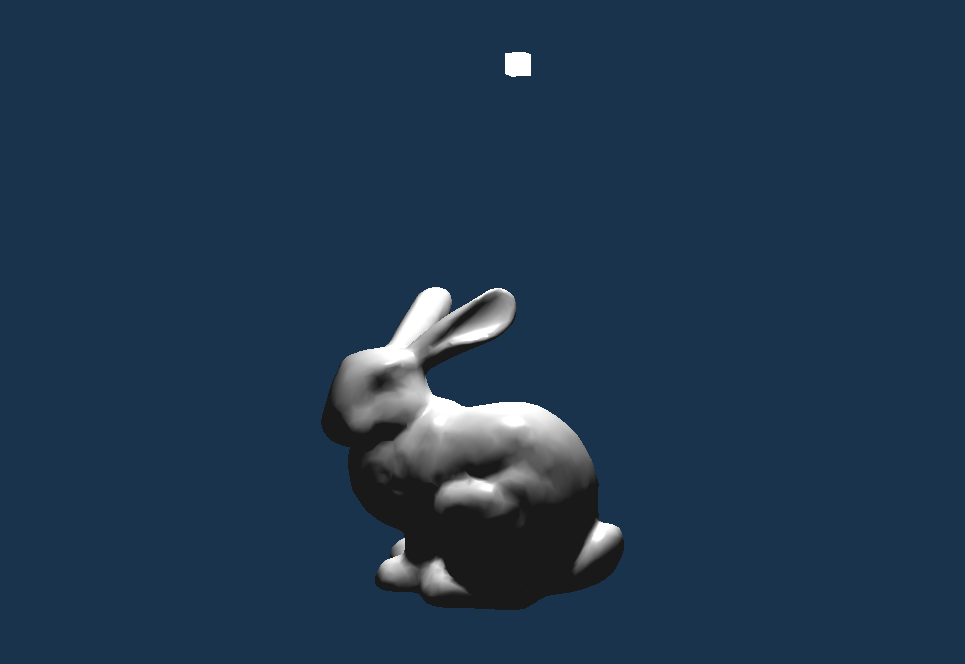
\includegraphics[scale=0.1]{Point Light Front.png}
		\end{minipage}
	}
	\subfigure[Back]
	{
		\begin{minipage}[b]{.4\linewidth}
			\centering
			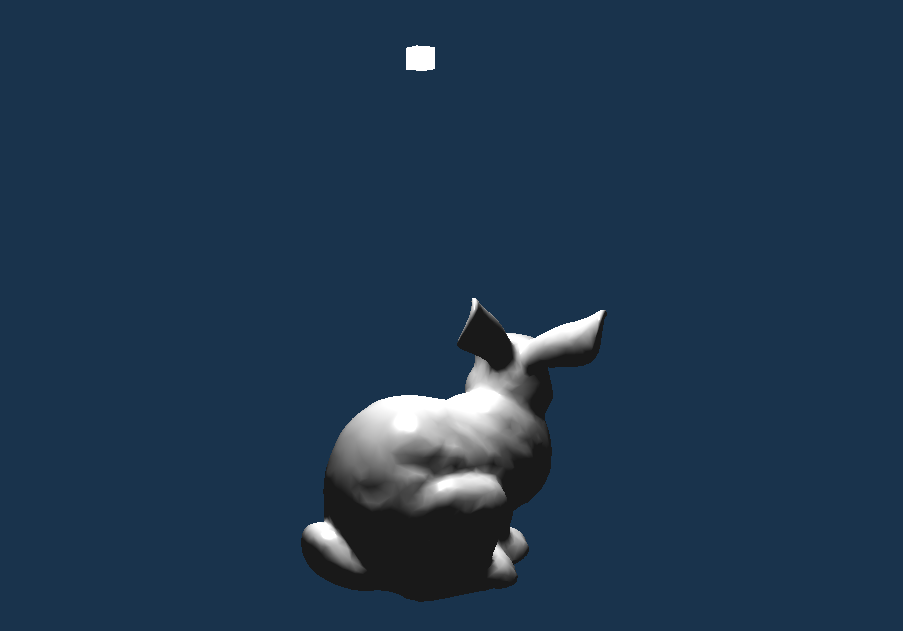
\includegraphics[scale=0.106]{Point Light Back.png}
		\end{minipage}
	}
	\caption{Point Light}
\end{figure}
\begin{figure}[h]
	\centering
	\subfigure[Front]
	{
		\begin{minipage}[b]{.4\linewidth}
			\centering
			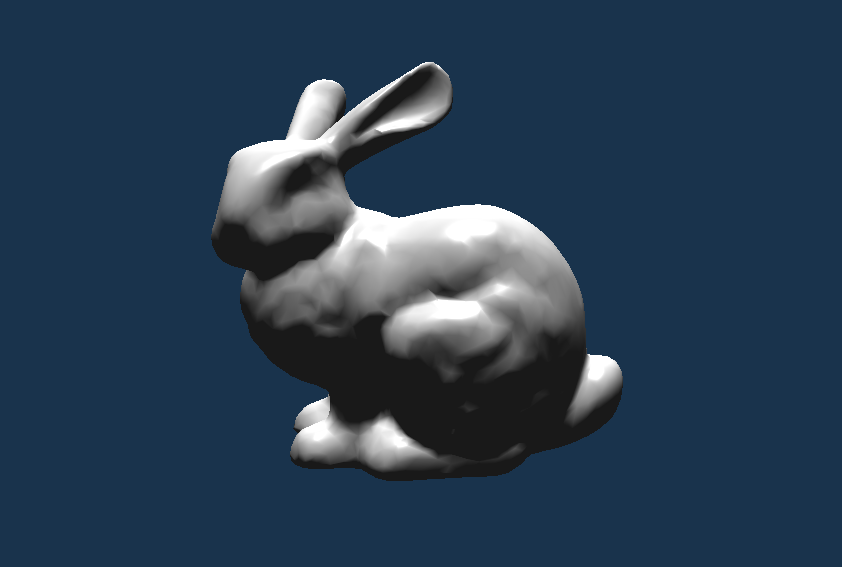
\includegraphics[scale=0.113]{Dirational Light Front.png}
		\end{minipage}
	}
	\subfigure[Back]
	{
		\begin{minipage}[b]{.4\linewidth}
			\centering
			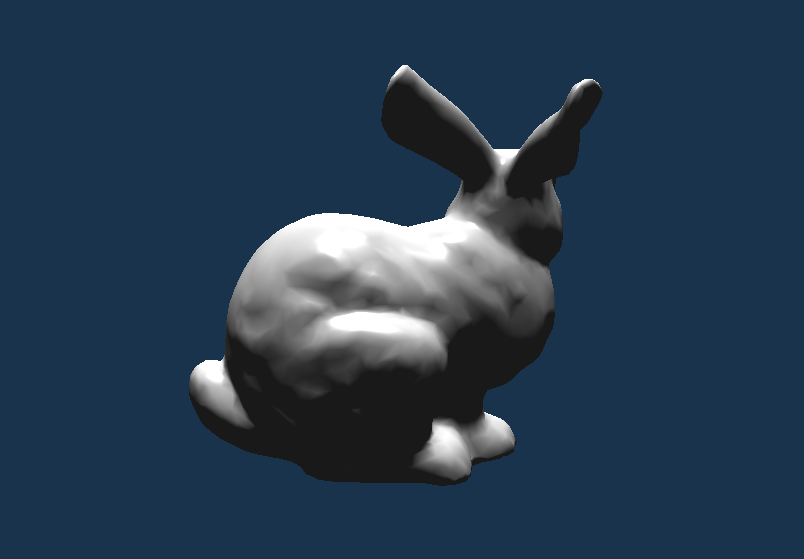
\includegraphics[scale=0.114]{Dirational Light Back.png}
		\end{minipage}
	}
	\caption{Directional Light}
\end{figure}
\begin{figure}
	\centering
	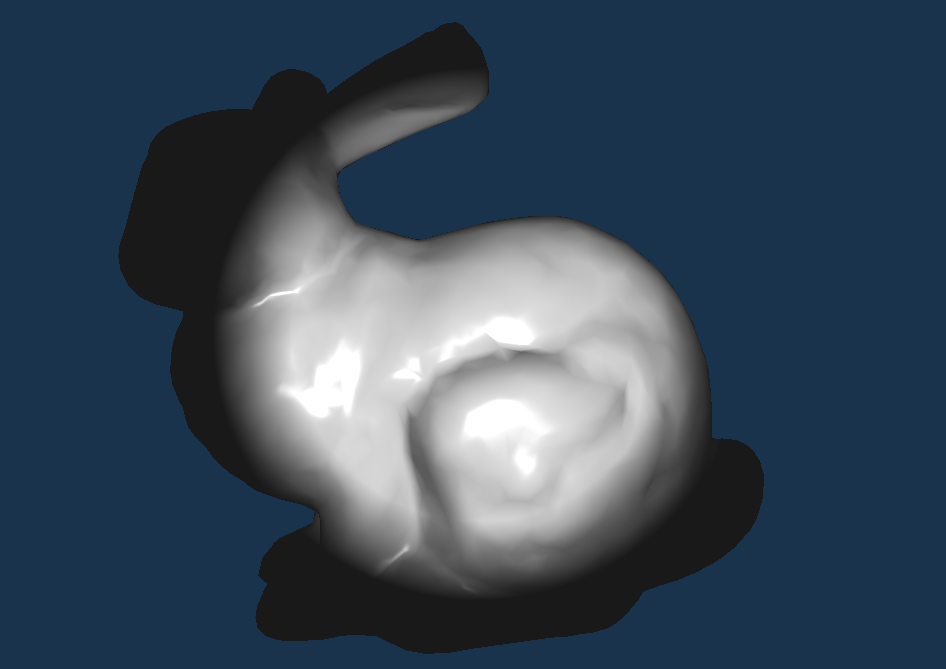
\includegraphics[scale=0.2]{Flashlight.png}
	\caption{Flashlight}
\end{figure}

\end{document}
